\chapter{Results and Discussions}

This chapter presents a comprehensive evaluation and validation of the security implementation mechanisms detailed in Section \ref{sec:sec_impl}. We systematically examine multiple security aspects through various testing procedures, including evaluating authentication mechanisms, conducting OIDC PKCE compliance tests, identifying cloud vulnerabilities, performing password hash compare timing tests, and assessing access control mechanisms. The investigation meticulously documents and analyses the empirical results, revealing the strengths and potential vulnerabilities of the implemented security framework.


\section{Manual Testing}
As a pre-condition for testing the two PKCE endpoints, a build script (refer to Appendix \ref{apendix:build_and_run_script}) is executed. This build script creates the required infrastructure by running the terraform, like the lambdas and API gateways. In addition to providing the infrastructure, the database will be seeded with two tenants and some users. In this section, manual tests of the two endpoints implemented are documented.


\subsection{Authorise Endpoint}
Manual tests were conducted on the \textbf{/authorize} endpoint to assess its functionality and security measures. The testing process included the following scenarios:

\begin{enumerate}
     \item \textbf{Successful Authentication:} Verified that the endpoint correctly processes authentication requests when provided with valid credentials, a valid client ID, and a proper code challenge. Additionally, the test was repeated successfully using \textbf{Tenant 2} to ensure multi-tenant compatibility. Figure \ref{fig:authorize_tenant_1_success} shows the successful authentication of a user in \textit{tenant 1} when all the required parameters and the credentials are correct, and Figure \ref{fig:authorize_tenant_1_wrong_pass} presents a successful authentication with \textit{tenant 2}.

\begin{figure}[!htbp]
    \centering
    \begin{lstlisting}[style=curlstyle]
Request:
curl -X POST http://tenant1.local:4566/restapis/o4qbjcrrti/dev/_user_request_/
authorize\
-H "Content-Type: application/json" \
-d '{"username": "user7@example.com","client_id":"tenant1-client-id-1", "password": "test1"}'

Response:{
"message":"Hello, user7@example.com",
"authorizationCode":{"S":"22f51d86-c29b-49ef-a594-9916d10a7617"},
"expiresAt":{"N":"1734690017"}
}
    \end{lstlisting}
    \caption{Successful user Authorise for tenant1}
    \label{fig:authorize_tenant_1_success}
\end{figure}


\begin{figure}[!htbp]
    \centering
    \begin{lstlisting}[style=curlstyle]
Request:
curl -X POST http://tenant2.local:4566/restapis/o4qbjcrrti/dev/_user_request_/authorize \                                  
-H "Content-Type: application/json" \
-d '{"username": "user7@example.com","client_id":"tenant2-client-id-1", "password": "test2", "codeChallenge": "ChX9V18izIUew6V7-DRS4hMRK3H_tlPBQ5E_umRHLNo"}'

Response:{
"message":"Hello, user7@example.com",
"authorizationCode":{"S":"79641e2f-2a32-46ef-9e61-263ba620acff"},
"expiresAt":{"N":"1734693110"}
}
    \end{lstlisting}
    \caption{Successful user Authorise for tenant2}
    \label{fig:authorize_tenant_2_success}
\end{figure}

\newpage
    \item \textbf{Authentication Failures:} Tested various failure scenarios to ensure the system handles them securely and as expected:
    \label{subsec:auth_failure_tests}
    \begin{itemize}
        \item \textbf{Invalid Credentials:} Attempted authentication with incorrect tenant credentials to confirm that the system denies access and provides appropriate error responses. Figure \ref{fig:authorize_tenant_1_wrong_pass} illustrates the denial of access that occurs when a user provides a wrong password.

        \begin{figure}[!htbp]
    \centering
    \begin{lstlisting}[style=curlstyle]
Request:
curl -X POST http://tenant2.local:4566/restapis/o4qbjcrrti/dev/_user_request_/authorize \                                  
-H "Content-Type: application/json" \
-d '{"username": "user7@example.com","client_id":"tenant2-client-id-1", "password": "wrong_password", "codeChallenge": "ChX9V18izIUew6V7-DRS4hMRK3H_tlPBQ5E_umRHLNo"}'

Response:{
"message":"Invalid username or password"}
}
    \end{lstlisting}
    \caption{Unsuccessful user Authorise for tenant1 with wrong password}
    \label{fig:authorize_tenant_1_wrong_pass}
\end{figure}

        

       
        \item \textbf{Unknown Client ID:} Tested requests with an unregistered or invalid client ID to confirm the endpoint rejects such requests without further processing. Figure \ref{fig:authorize_tenant_1_unknown_client} depicts the curl request with \textit{tenant 1}
        and an unknown \textit{client\_id}, and responds with access deined with a corresponding error message.

\begin{figure}[!htbp]
    \centering
    \begin{lstlisting}[style=curlstyle]
Request:
curl -X POST http://tenant1.local:4566/restapis/o4qbjcrrti/dev/_user_request_/authorize \                                  
-H "Content-Type: application/json" \
-d '{"username": "user7@example.com","client_id":"unknown-client-id-1", "password": "test2", "codeChallenge": "ChX9V18izIUew6V7-DRS4hMRK3H_tlPBQ5E_umRHLNo"}'

Response: {"message":"Invalid client ID"}
    \end{lstlisting}
    \caption{Unsuccessful user Authorise for tenant1 with Unknown Client}
    \label{fig:authorize_tenant_1_unknown_client}
\end{figure}


    \end{itemize}
\end{enumerate}

These tests helped validate the robustness of the \textbf{/authorize} endpoint, ensuring it functions correctly under normal conditions while effectively mitigating common security threats.

\newpage
\subsection{Token Endpoint}
Manual tests were also conducted on the \textbf{/token} endpoint to verify its functionality and robustness. The following scenarios were tested:

\begin{enumerate}
    \item \textbf{Successful Token Retrieval:} Verified that the endpoint successfully issues tokens when provided with a valid authorisation code, client ID, and code verifier. The tokens are signed using an asymmetric key using the RS256 Algorithm (Refer to Figure \ref{fig:token_tenant_1_token_signed}). The private key is generated using the RSA-2048-bit algorithm (refer to Appendix \ref{apendix:create_private_keys}), and the keys are stored securely in the secrets manager, which the token lambda retrieves (Refer to Appendix \ref{apendix:token_signing}). Figure \ref{fig:token_tenant_1_success} illustrates a successful retrieval of an access token of a user after authentication.


        \begin{figure}[!htbp]
    \centering
    \begin{lstlisting}[style=curlstyle]
Request:
curl -X POST http://tenant1.local:4566/restapis/o4qbjcrrti/dev/_user_request_/token\                                      
-H "Content-Type: application/json" \
-d '{
    "username": "user7@example.com","grant_type": "authorization_code","client_id":"tenant1-client-id-1", "authorizationCode": "a24e5543-7ed6-4511-a021-be911004f187", "codeVerifier": "wOV-nI-            
    QSyesPpyjPpyjkBPx7PCimGUBrxOqKgc8idU
    NLnzeIkUq1nJI4R2hEyoolgexTqQfAd4hbX8mi
    7ud0BpQv16u6R9a14fWjXjj65uWDnV-nfI7Ow-YaippAChI
"}'

Response: {
    "token":"eyJhbGciOiJSUzI1NiIsInR5cCI6IkpXVC
    J9.eyJ1c2VySWQiOiJ1c2VyLTI2Mjc3LTEyMjc2IiwiaWF0
    IjoxNzM0NzAwNDg5LCJleHAiOjE3MzQ3MDQwODl9.NMjBNY
    w4rprZ_irSFv0MKWrIt3KiOtteNeDDvwlv-T2QMpcgIEfdT5
    Nvc_zjIOotayqiHHtQNBQf_j-Y89z52Sv-076UaQOq5SeEU52
    voaqUABAQ5QoaaTELmCWMDOovAK9_9fo
    sF0Am5hMYBZe3S8H0vUKqdSM1Bcu2ONAo40tRCowfK90NHp1q5A
    2CBuXanbCiVYrzZZ0Bes6y0Xpun6ldu8FnSIzgmzE3sPCGmmRP5E
    kE1IoW2ViQ4irklUkFWXBZDjoZZua9CoPzcgH0OWD_uL48ZqSiXO
    PbvO_TcKCZ5ORnHPdeN7PRupllUFaR-M9B4yZtfjujFBHBSi63A"
}
    \end{lstlisting}
    \caption{Successful token retrieval for tenant 1}
    \label{fig:token_tenant_1_success}
\end{figure}

\newpage
    \item \textbf{Expired Authorisation Code:} Attempted to retrieve a token using an expired authorisation code to ensure the endpoint denies the request with an appropriate error response. Figure \ref{fig:token_auth_code_expired} illustrates the denial of authority when the token endpoint is requested with an expired user \texttt{authorisation code}.
    
    
    \begin{figure}[!htbp]
    \centering
    \begin{lstlisting}[style=curlstyle]
Request:
curl -X POST http://tenant1.local:4566/restapis/o4qbjcrrti/dev/_user_request_/token\                                      
-H "Content-Type: application/json" \
-d '{
    "username": "user7@example.com","grant_type": "authorization_code","client_id":"tenant1-client-id-1", "authorizationCode": "a24e5543-7ed6-4511-a021-be911004f187", "codeVerifier": "wOV-nI-            
    QSyesPpyjPpyjkBPx7PCimGUBrxOqKgc8idU
    NLnzeIkUq1nJI4R2hEyoolgexTqQfAd4hbX8mi
    7ud0BpQv16u6R9a14fWjXjj65uWDnV-nfI7Ow-YaippAChI
"}'

Response: {"message":"Invalid authorization code or code verifier or expired"}
    \end{lstlisting}
    \caption{Unsuccessful token retrieval as Authorisation Code expired}
    \label{fig:token_auth_code_expired}
\end{figure}
\end{enumerate}

\noindent These tests validated the \textbf{/token} endpoint's ability to securely handle both successful and invalid requests, ensuring proper error handling for edge cases and enforcement of PKCE requirements.

\newpage
\subsection{PKCE Downgrade Tests}
\begin{enumerate}

    \item \textbf{Missing Code Verifier:} We conducted a simulation in which we omitted the \texttt{code\_verifier}  parameter during the token exchange process. This test demonstrated that the endpoint rejects the request appropriately, ensuring compliance with PKCE (Proof Key for Code Exchange). In Figure \ref{fig:token_no_code_veri}, we show the PKCE Downgrade attack, demonstrating how the system denies the token request because it lacks the \texttt{code\_verifier}. This request's denial proves that one cannot retrieve the token without the verifier parameter.

        \begin{figure}[!htbp]
    \centering
    \begin{lstlisting}[style=curlstyle]
Request:
curl -X POST http://tenant1.local:4566/restapis/o4qbjcrrti/dev/_user_request_/token\                                      
-H "Content-Type: application/json" \
-d '{
    "username": "user7@example.com","grant_type": "authorization_code","client_id":"tenant1-client-id-1", "authorizationCode": "a24e5543-7ed6-4511-a021-be911004f187"}'

Response: {"message":"Missing 'username', 'authorizationCode', or 'codeVerifier' in request body"}
    \end{lstlisting}
    \caption{Unsuccessful token retrieval as no Code Verifier Present (PKCE Downgrade)}
    \label{fig:token_no_code_veri}
\end{figure}

    \item \textbf{Missing Code Challenge:} Simulated a PKCE (Proof Key for Code Exchange) downgrade attack by omitting the \texttt{code\_challenge} parameter. This test was designed to ensure that the endpoint enforces PKCE requirements and denies the request if missing the \texttt{code\_challenge}. In Figure \ref{fig:authorize_tenant_1_without_code_challenge}, we show the PKCE Downgrade attack, demonstrating how the system denies the authorise request because it lacks the \texttt{code\_challenge}. 


        \begin{figure}[!htbp]
    \centering
    \begin{lstlisting}[style=curlstyle]
Request:
curl -X POST http://tenant1.local:4566/restapis/o4qbjcrrti/dev/_user_request_/authorize \                                  
-H "Content-Type: application/json" \
-d '{"username": "user7@example.com","client_id":"tenant1-client-id-1", "password": "test1"}'

Response: {"message":"Invalid request body"}
    \end{lstlisting}
    \caption{Unsuccessful user Authorise for the tenant1 without Code Challenge (PKCE Downgrade)}
    \label{fig:authorize_tenant_1_without_code_challenge}
\end{figure}

    \newpage
    \item \textbf{Missing Grant Type:} Sent a token exchange request without setting  \sloppy \seqsplit{grant\_type=authorization\_code}, confirming that the endpoint validates the presence of required parameters and returns a proper error if the \texttt{grant\_type} is missing or incorrect.In Figure \ref{fig:token_no_grant_type}, we show the PKCE Downgrade attack, demonstrating how the system denies the token request because it lacks the \texttt{grant\_type}.


                \begin{figure}[!htbp]
    \centering
    \begin{lstlisting}[style=curlstyle]
Request:
curl -X POST http://tenant1.local:4566/restapis/o4qbjcrrti/dev/_user_request_/token\                                      
-H "Content-Type: application/json" \
-d '{
    "username": "user7@example.com",
    "client_id":"tenant1-client-id-1", "authorizationCode": "a24e5543-7ed6-4511-a021-be911004f187",
    "codeVerifier": "wOV-nI-QSyesPpyjPpyjkBPx7PCimGUBrxOqKgc8idUNLnzeIkU
    q1nJI4R2hEyoolgexTqQfAd4hbX8mi7ud0BpQv16u6R9
    a14fWjXjj65uWDnV-nfI7Ow-YaippAChI"
    }'

Response: {"message":"Invalid Grant Type"}
    \end{lstlisting}
    \caption{Unsuccessful token retrieval as no Grant Type (PKCE Downgrade)}
    \label{fig:token_no_grant_type}
\end{figure}
\end{enumerate}
       


\subsection{Timing Safe Function Test}
\label{sec:timing_test}
Table \ref{table:sec_impl} emphasises that the timing-safe functions of Argon2id were employed to compare hashes, mitigating the risk of side-channel attacks, specifically timing attacks. To verify the robustness of these functions against information leakage, a test was conducted involving 1000 timing measurements for two scenarios: hash comparisons using random, incorrect passwords and comparisons with the correct password. Appendix \ref{apendix:timing_test} presents the code that executes to collect the timing samples and calculate the p-value. The truncated results of these measurements are presented in Tables \ref{table:non_matching_pass_res} and \ref{table:matching_pass_res}.

The recorded timings show slight variations across runs due to inherent measurement noise. Pearson's $\chi^2$ test (chi-squared) was conducted to assess whether this noise could lead to a side-channel attack. As supported by \cite{chisquare}, this statistical method effectively evaluates if the system's noise is sufficient to prevent timing-related information leakage. The $\chi^2$ test compares the observed timing distribution against an expected random distribution, quantitatively measuring the system's resilience to timing attacks. This approach offers a more rigorous and statistically grounded assessment of the system's security against potential timing-based vulnerabilities.

To perform the $\chi^2$ test, the following null and alternative hypotheses are set:
\begin{itemize}
    \item \textbf{Null Hypothesis} - H$0$: $\mu1 = \mu2$ (Where the mean of sample 1 equals the mean of sample 2).
    \item \textbf{Alternate Hypothesis} - H$1$: $\mu1 \neq \mu2$  (Where two sample means are different).   
    \item \textbf{Statistical Significance Level} - An Alpha ($\alpha$) of 5\% or 0.05 is chosen, which, if the p-value is less than this value, the null hypothesis will be rejected. 
\end{itemize}

The function presented in Listing \ref{lst:chisqrd} is utilised to compute the chi-square statistic and the corresponding p-value for the provided samples.
By applying this function, a p-value of 0.98 is obtained.
This result indicates that we do not reject the null hypothesis, suggesting that the likelihood of information leakage due to timing attacks is minimal, thereby offering a means to mitigate such side-channel attacks.

\begin{lstlisting}[style=typescript,caption=Chi-Squared Function Written in Typescript ,label=lst:chisqrd]
const calculateChiSquare = (sample1: number[], sample2: number[]) => {
    const degreesOfFreedom = sample1.length - 1;
    const chiSquared = sample1.reduce((sum, obs, i) => {
        const exp = sample2[i];
        return sum + Math.pow(obs - exp, 2) / exp;
    }, 0);
    const pValue = 1 - jstat.chisquare.cdf(chiSquared, degreesOfFreedom);
    return {chiSquared, pValue, degreesOfFreedom};
}
\end{lstlisting}

\begin{longtable}{|c|c|}
\caption{Truncated Timing Samples for the Hash Comparison for an Incorrect Password (in ms)}
\label{table:non_matching_pass_res}
\hline
\rowcolor{grey!15}
\textbf{Index} & \textbf{Values}      \\ \hline
\endfirsthead
\hline
\rowcolor{grey!15}
\textbf{Index} & \textbf{Values}      \\ \hline
\endhead
\hline
\endfoot
\hline
\endlastfoot
0              & 162.13    \\ \hline
1              & 161.73   \\ \hline
2              & 157.79   \\ \hline
3              & 158.16   \\ \hline
4              & 152.18    \\ \hline
5              & 149.70   \\ \hline
6              & 154.48   \\ \hline
7              & 150.59   \\ \hline
8              & 149.33   \\ \hline
9              & 161.63    \\ \hline
10             & 161.07   \\ \hline
\multicolumn{2}{|c|}{...}             \\ \hline
\end{longtable}



\begin{longtable}{|c|c|}
\caption{Truncated Timing Samples for the Hash Comparison for a Correct Password (in ms)}
\label{table:matching_pass_res}
\hline
\rowcolor{grey!15}
\textbf{Index} & \textbf{Values}      \\ \hline
\endfirsthead
\hline
\rowcolor{grey!15}
\textbf{Index} & \textbf{Values}      \\ \hline
\endhead
\hline
\endfoot
\hline
\endlastfoot
0              & 142.11    \\ \hline
1              & 150.21   \\ \hline
2              & 152.93    \\ \hline
3              & 151.94   \\ \hline
4              & 148.29   \\ \hline
5              & 147.69   \\ \hline
6              & 148.18   \\ \hline
7              & 149.09    \\ \hline
8              & 149.97   \\ \hline
9              & 150.53   \\ \hline
10             & 150.41   \\ \hline
\multicolumn{2}{|c|}{...}             \\ \hline
\end{longtable}


\subsection{Automated Tests And Scans}
In addition to manual tests, various automated tests and security scans were conducted to ensure the application's robustness, security, and maintainability. The automated testing process included:

\begin{enumerate}
    \item \textbf{Unit Tests:} 
    Automated unit tests were implemented to validate the functionality of individual components of the \textbf{/authorize} and \textbf{/token} endpoints. These tests ensure that each component operates as intended, providing confidence in the correctness and reliability of the code. 

    The unit tests covered both the positive and negative scenarios for the business logic of the endpoints, verifying that:
    \begin{itemize}
        \item The \textbf{/authorize} endpoint correctly handles authentication requests, validates input parameters and securely generates authorisation codes.
        \item The \textbf{/token} endpoint properly exchanges authorisation codes for access tokens, enforces PKCE compliance and handles edge cases, such as expired or invalid codes.
    \end{itemize}
    
    As illustrated in Figure~\ref{fig:Unit Test}, the unit tests achieved a code coverage of approximately 97\%. This high level of coverage indicates that nearly all the application's critical paths and edge cases were thoroughly tested, ensuring functional correctness and robustness.

        \begin{figure}[!htbp]
         \centering
         {\setlength{\fboxrule}{2pt} % Border thickness
         \setlength{\fboxsep}{1pt}  % Space between image and border
         \fbox{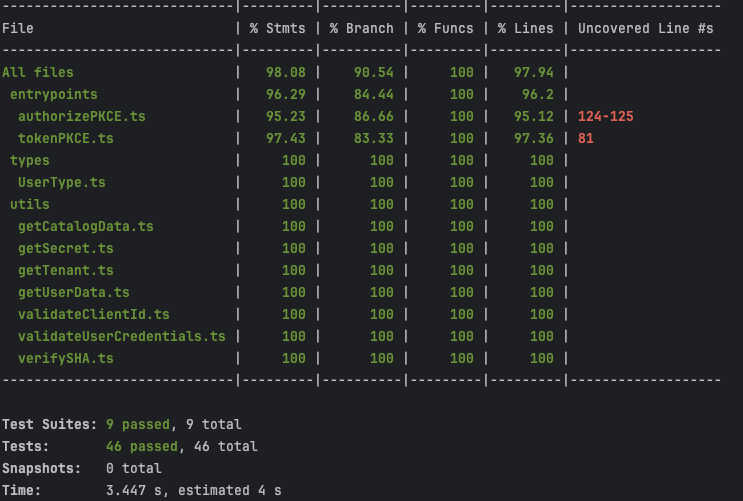
\includegraphics[width=\textwidth, height=200px]{pics/unit_test.png}} % Image with border
        \caption{Results of the Unit Test for the PKCE Prototype in Localstack}
        \label{fig:Unit Test}
    \end{figure}

    \item \textbf{Fuzz Tests:} 
    Fuzz testing was conducted by sending random or malformed input to the \textbf{/token} endpoint to identify potential vulnerabilities, such as crashes, unexpected behaviour, or unhandled exceptions. This helps ensure the endpoint is resilient to invalid or malicious inputs.

    \item \textbf{Security Scans:}
    Security scans were employed to identify potential vulnerabilities and maintain best practices:
    \begin{itemize}
        \item \textbf{Code Linting with ESLint:} 
        ESLint was utilised to identify code smells and ensure the codebase adhered to clean coding principles and established security best practices. Linting is crucial in minimizing the risk of introducing vulnerabilities by enforcing consistent code quality. The eslint-plugin-security-node plugin was used to enhance this process, which proved to be highly effective in detecting common security issues and code smells. Its integration ensured a more robust and secure codebase by proactively addressing potential weaknesses. Figure \ref{fig:lint_results} depicts the results of some code smells detected using the linter. 

                \begin{figure}[!htbp]
                     \centering
                     {\setlength{\fboxrule}{2pt} % Border thickness
                     \setlength{\fboxsep}{1pt}  % Space between image and border
                     \fbox{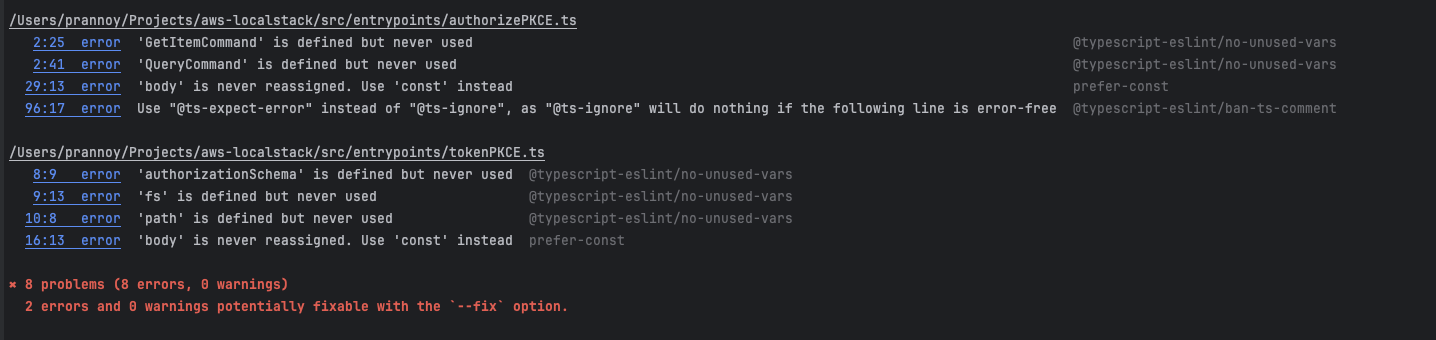
\includegraphics[width=\textwidth, height=180px]{pics/linting.png}} % Image with border
                    \caption{Lint results}
                    \label{fig:lint_results}
                \end{figure}


        \item \textbf{Cloud Infrastructure Scanning with Prowler:} 
        Prowler is a versatile open-source tool designed to scan cloud providers like AWS, helping identify potential misconfigurations in cloud infrastructure. It provides critical insights into security risks, such as overly permissive IAM roles, improper or missing logging configurations, and inadequate encryption settings. One of the critical strengths of Prowler is its ability to not only detect these issues but also provide actionable recommendations and remedies to address the identified misconfigurations. For example, as shown in Figure \ref{fig:prowler_results}, the tool detected 14 medium-level misconfigurations, each accompanied by specific remediation steps to mitigate the associated risks.

                \begin{figure}[!htbp]
                     \centering
                     {\setlength{\fboxrule}{2pt} % Border thickness
                     \setlength{\fboxsep}{1pt}  % Space between image and border
                     \fbox{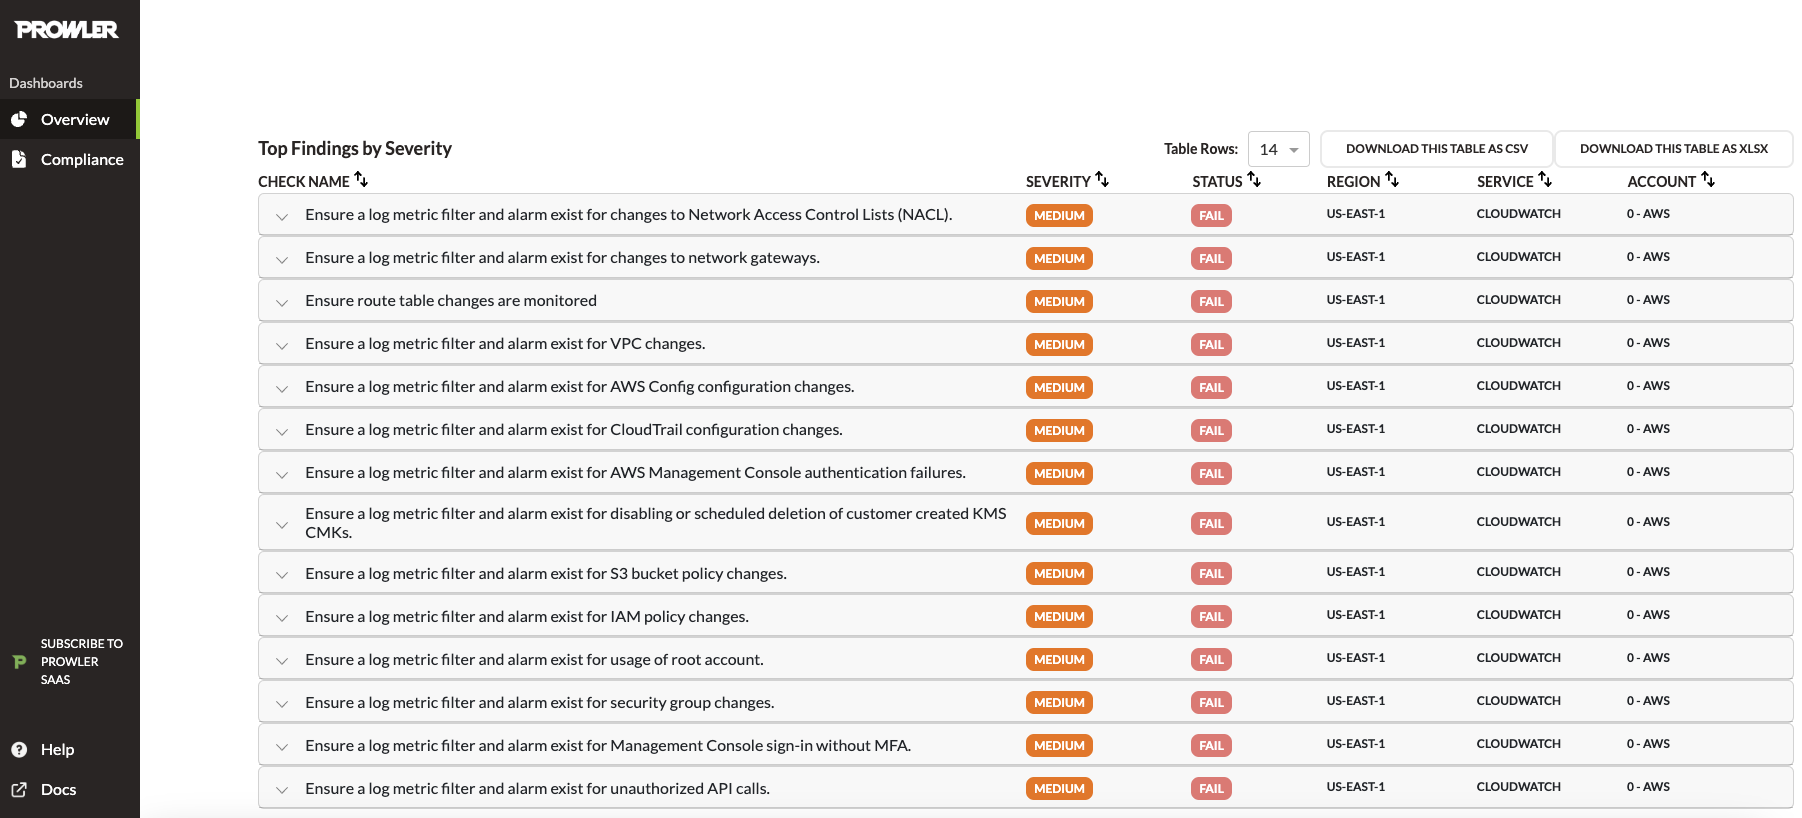
\includegraphics[width=\textwidth, height=120px]{pics/prowler.png}} % Image with border
                    \caption{Prowler Scan result}
                    \label{fig:prowler_results}
                \end{figure}

        
        In addition to the standard security checks, Prowler extends its functionality to compliance auditing. It supports testing against various industry standards, offering organisations a way to assess and strengthen their compliance posture. In this context, Prowler was utilised to perform both cloud infrastructure scans and compliance checks for ISO 27001:2013 (refer to Figure \ref{fig:prowler_iso_results}) and GDPR (refer to Figure \ref{fig:prowler_gdpr_results}). These compliance scans are particularly valuable for organisations that adhere to regulatory requirements or maintain certifications, as they provide a comprehensive view of potential gaps and actionable insights for achieving compliance.
        
                \begin{figure}[!htbp]
                     \centering
                     {\setlength{\fboxrule}{2pt} % Border thickness
                     \setlength{\fboxsep}{1pt}  % Space between image and border
                     \fbox{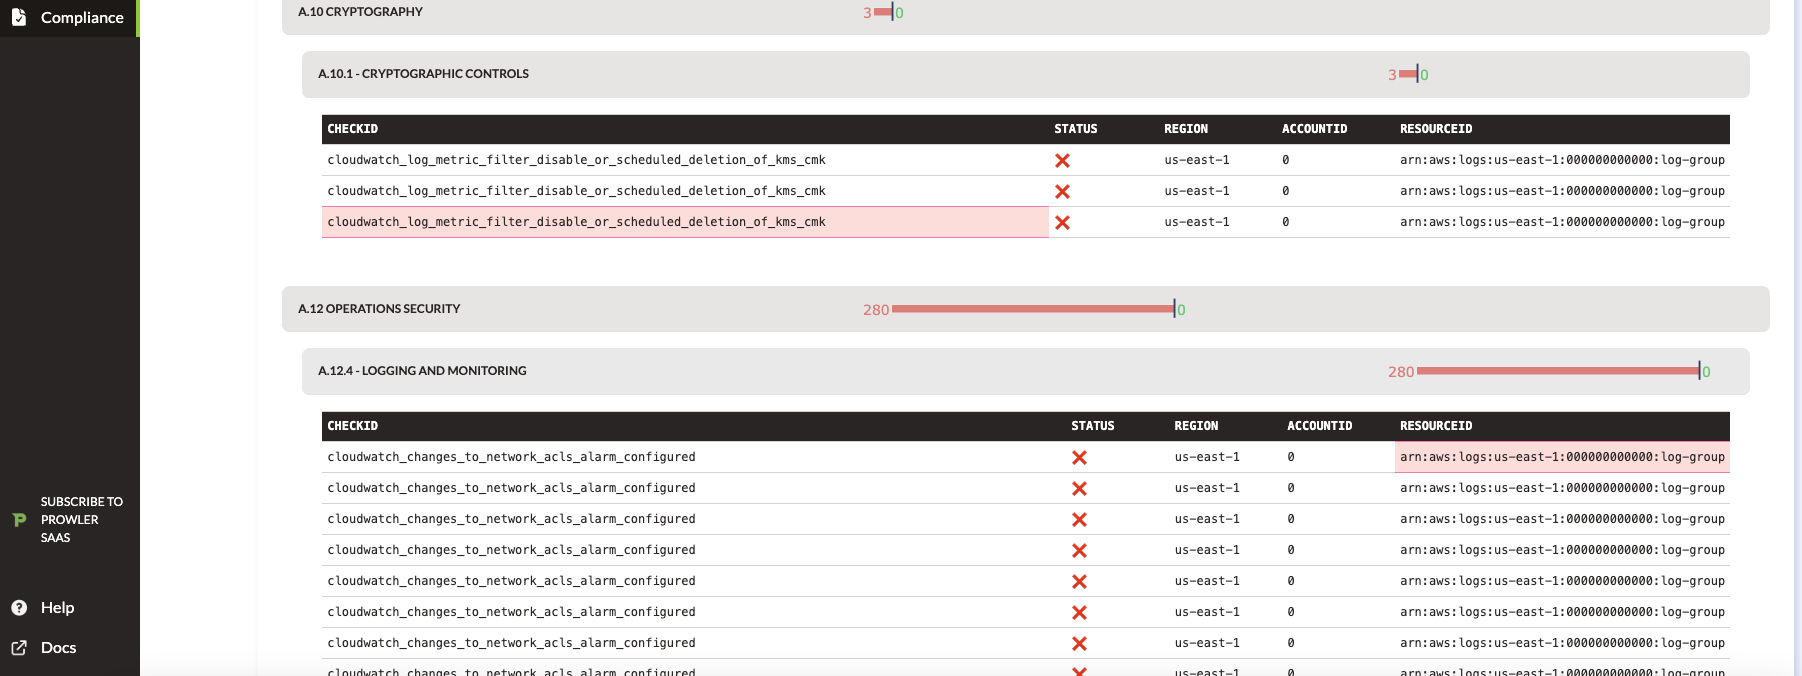
\includegraphics[width=\textwidth, height=150px]{pics/prowler_iso.png}} % Image with border
                    \caption{Prowler ISO:27001:2013 Scan result}
                    \label{fig:prowler_iso_results}
                \end{figure}

                \begin{figure}[!htbp]
                     \centering
                     {\setlength{\fboxrule}{2pt} % Border thickness
                     \setlength{\fboxsep}{1pt}  % Space between image and border
                     \fbox{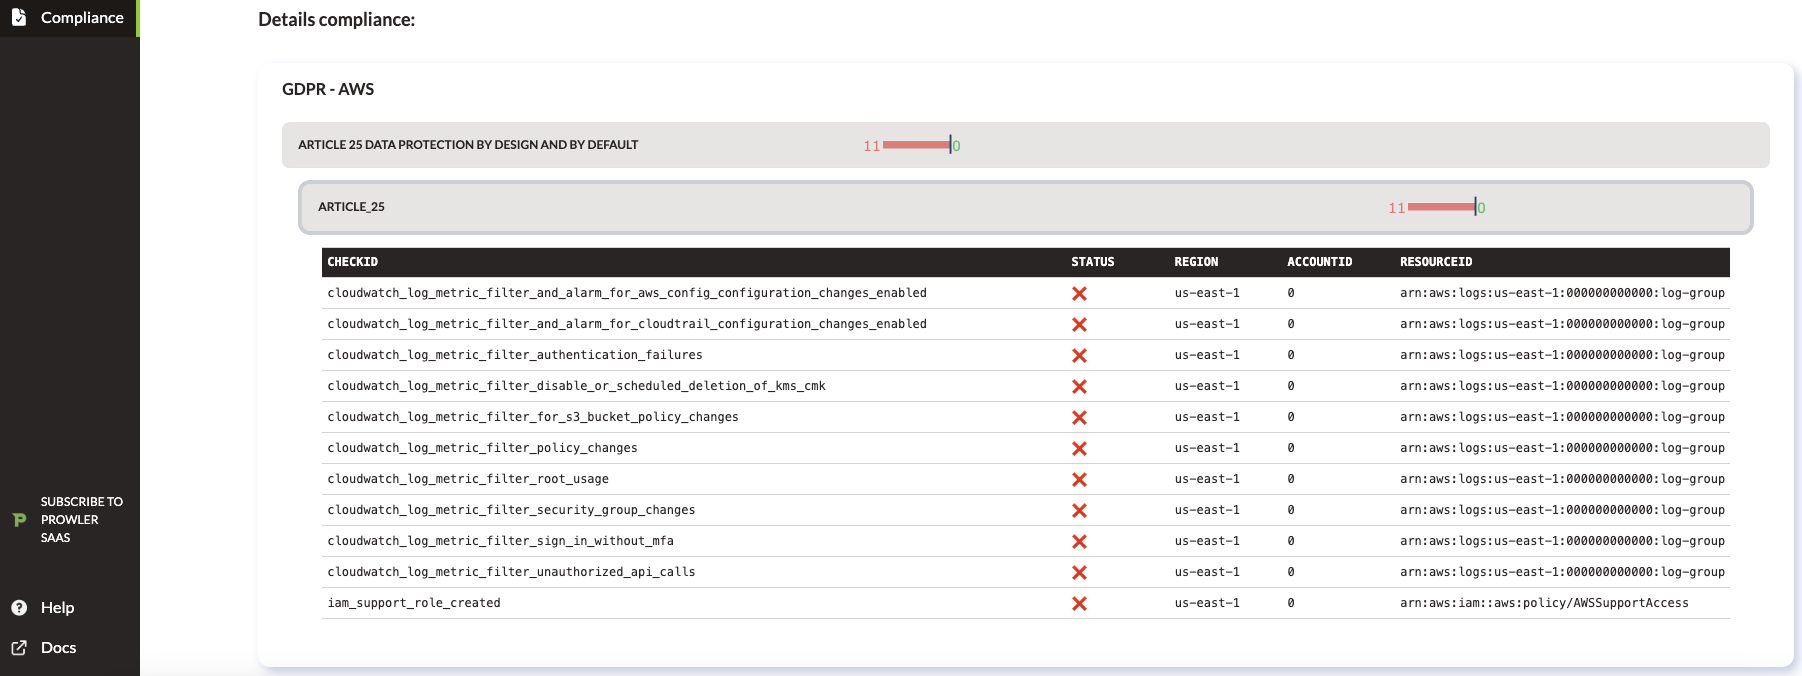
\includegraphics[width=\textwidth, height=150px]{pics/prowler_gpdr.png}} % Image with border
                    \caption{Prowler GDPR Scan result}
                    \label{fig:prowler_gdpr_results}
                \end{figure}
        By integrating security scanning with compliance testing, Prowler is a powerful tool for proactively securing cloud environments and aligning with best practices.        
    \end{itemize}
    \item \textbf{Static Code Analysis with Snyk:} Snyk is utilised in this project as a static analysis tool to detect vulnerabilities, improve code quality, and ensure secure development practices. It complements \texttt{ESLint} by focusing on security flaws in business logic and Infrastructure-as-Code (IaC). While \texttt{ESLint} enforces coding standards and detects bugs in JavaScript, Snyk extends the scope by scanning for vulnerabilities in dependencies, IaC configurations, and container images. This integration ensures both high-quality code and robust security measures. Figure \ref{fig:snyk_results} illustrates the results of Snyk's analysis.
    

    \begin{figure}[!htbp]
                     \centering
                     {\setlength{\fboxrule}{2pt} % Border thickness
                     \setlength{\fboxsep}{1pt}  % Space between image and border
                     \fbox{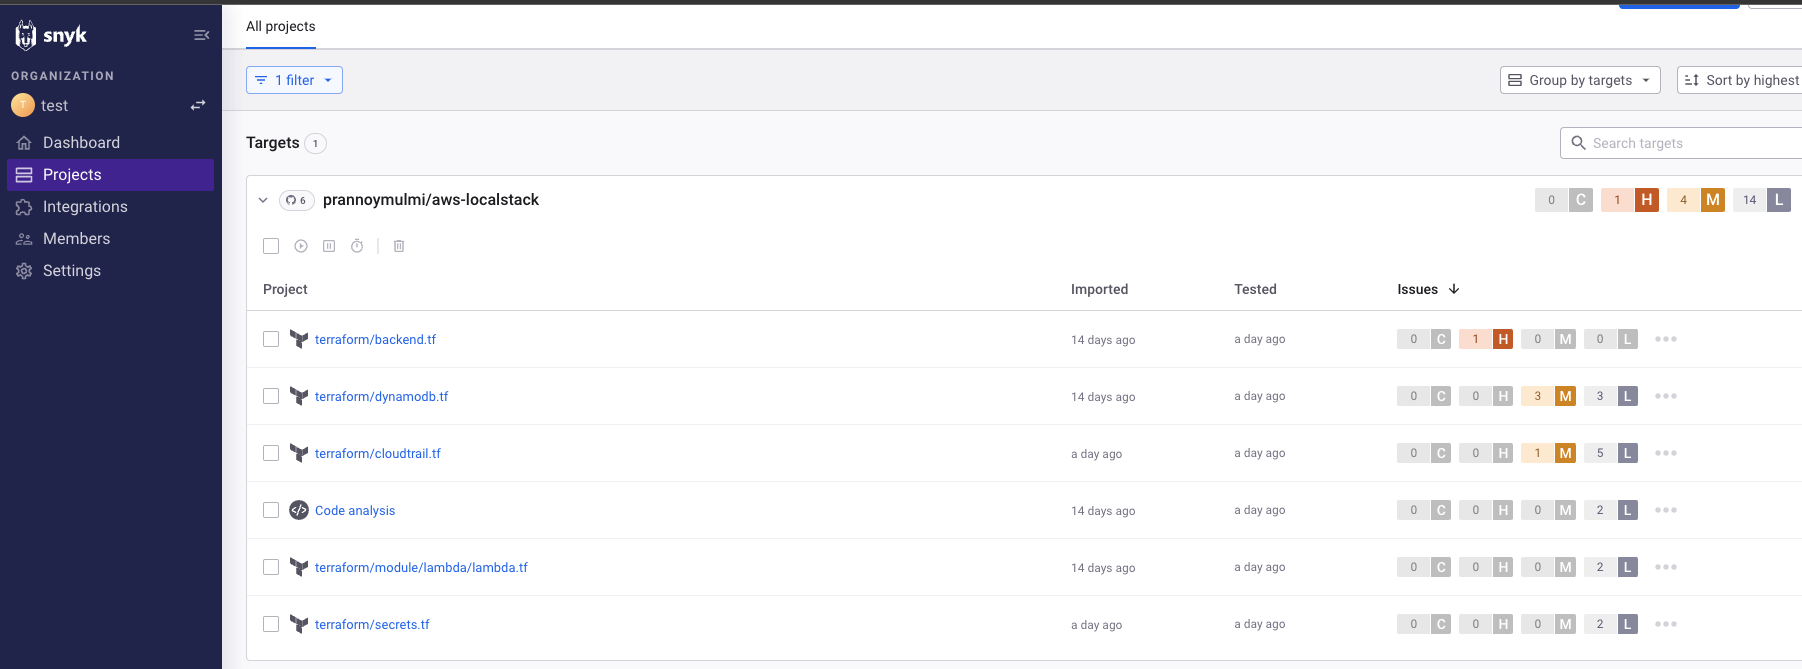
\includegraphics[width=\textwidth]{pics/snyk.png}} % Image with border
                    \caption{Static Code Analysis with Snyk}
                    \label{fig:snyk_results}
                \end{figure}
\end{enumerate}

\newpage
\subsection{Test Summary}
\begin{longtable}{|p{5cm}|p{10cm}|}
\hline
\rowcolor{grey!15}
\textbf{Threat} & \textbf{Test} \\
\hline
\endhead
\hline
\endfoot
Cloud Misconfigurations &  Figures \ref{fig:prowler_results} and \ref{fig:snyk_results} presents test results from Prowler and Snyk that identify several cloud misconfigurations. These tools revealed various configuration improvements that could threaten this application, providing valuable information. \\
\hline
Cross-Tenant Data Leakage & Integration tests were conducted using the tenant1 domain name to access user data from tenant 2. The tenant1 domain name limits the access to data only from tenant one. Listing \ref{apendix:cross_tenant_data_integ_test} shows the tests using the client ID of tenant two and using user credentials that belong to tenant 1. These tests both resulted in a denial of the request.\\
\hline
Code Injection (XSS, SQLi) \& Code Vulnerabilities & \begin{itemize}
    \item Unit tests were carried out where inputs of length less than 43 and more than 128 were provided. These tests rejected the requests that stood outside this range. For the implementation code, refer to Appendix \ref{apendix:rfc7636_test}.
    \item Fuzz test that inputs various random strings to detect unusual behaviour of the system. Refer to Appendix \ref{apendix:fuzz_test} to see the implementation of the fuzz tests that use different random inputs on the authorise endpoint.
\end{itemize}\\
\hline
 Unauthorised Access & Manual testing, and unit testing have been conducted where using expired authorisation code, invalid credentials, use of invalid client\_id, and invalid code\_verifier has been tested. During all the tests, access was denied, and neither the authorisation code nor the access token was issued. Refer to the Manual Testing Section \ref{subsec:auth_failure_tests} to see the results for denied access for the mentioned cases.\\
\hline
PKCE Downgrade Attack & To test the PKCE Downgrade attack, a manual authorisation request was created without a code\_challenge. During this test, the authorisation server rejected all the requests without hashed code\_challenge or missing code\_verifier. Refer to Figure \ref{fig:authorize_tenant_1_without_code_challenge} where a PKCE Downgrade attack without code\_challenge was executed.\\
\hline
Timing Attacks & A test recording the compute time to verify 1000 samples of wrong passwords and 1000 samples of correct passwords were recorded. A Pearson’s $X^{2}$ test was then performed to assess leakage detection with the two sample sets. Refer to Section \ref{sec:timing_test} for the statistical test performed and the results.\\
\hline
\end{longtable}

\section{Results} 

\subsection{Cloud Configuration: A Top Security Concern}

In this analysis, the misconfiguration of cloud services emerged as one of the most significant issues. This finding was supported by vulnerability scans conducted using \textbf{Prowler} and \textbf{Snyk}, which identified multiple configuration-related warnings and vulnerabilities across the actively used cloud services: \textbf{Amazon DynamoDB}, \textbf{Amazon API Gateway (APIGW)}, and \textbf{AWS Lambda}.

\paragraph{Security Scan Results}
\begin{itemize}
    \item \textbf{Prowler}: Prowler flagged \textbf{14 medium-severity warnings} and \textbf{1 high-severity warning} within the scanned cloud configurations. These issues highlight potential risks that could expose the environment to unauthorised access or reduce its resilience to attacks.
    \item \textbf{Snyk}: Snyk detected \textbf{1 high-severity issue}, \textbf{4 medium-severity vulnerabilities}, and \textbf{1 low-severity issue}. These findings further corroborate the need for a robust approach to managing cloud configuration risks.
\end{itemize}

\paragraph{Complexity and Scaling Risks}:
The scans were conducted for only three actively used AWS services: \textbf{DynamoDB}, \textbf{APIGW}, and \textbf{Lambda}, which represent a subset of a typical cloud environment. Despite the limited scope, the results already highlight significant concerns about misconfiguration. As the number of services grows and their interdependencies increase, the complexity of managing cloud configurations will scale significantly. This growth will likely lead to an even greater risk of misconfigurations, amplifying the potential attack surface.

Following the finding, it is necessary to emphasize that \textbf{cloud configurations represent a critical security threat}. This aligns with the assessment outlined in \ref{table:threat_model_assets}, where misconfiguration was identified as one of the top-ranked threats to the cloud environment. Misconfigured resources can lead to data breaches, service disruptions, and compliance violations, underscoring the importance of proactive configuration management and continuous monitoring.

\newpage
\subsection{Security Tools: Useful but Not Sufficient}

Security tools such as \textbf{Prowler} and \textbf{Snyk} provide valuable insights into potential vulnerabilities and misconfigurations within cloud environments. However, while these tools are effective for identifying numerous issues, they cannot be solely relied upon for ensuring a secure setup. Several limitations and shortcomings were observed during the analysis, highlighting the importance of complementing automated tools with reviews from an expert and adherence to security best practices.

\paragraph{Undetected Security Issues}

Despite their advantages, the tools failed to detect certain critical issues deliberately introduced into the environment for testing purposes. These include:

\begin{itemize}
    \item \textbf{IAM Policy Not Following the Principle of Least Privilege}: 
    A deliberately misconfigured IAM policy that violated the principle of least privilege (refer to Listing \ref{lst:bad_policy_iam}) was created as part of the test. Such a policy, if accessed by a malicious actor, could be exploited to gain elevated privileges and compromise the environment. However, this misconfiguration or bad practice was not flagged by any of the tools used in this study.

    \begin{lstlisting}[caption={Added a Bad IAM Policy that allows all actions}, label={lst:bad_policy_iam}]
# IAM Policy for Lambda to log to CloudWatch
resource "aws_iam_policy" "test_bad_policy" {
  name        = "bad policy"
  description = "IAM policy test for bad example"

  policy = jsonencode({
    Version = "2012-10-17",
    Statement = [
      {
        Effect = "Allow",
        Action = [
          "*:*"
        ],
        Resource = "*"
      }
    ]
  })
}
\end{lstlisting} 

\item \textbf{False Positives and Contextual Irrelevance}: Besides undetected issues, the tools occasionally generated \textbf{false positives} or flagged findings irrelevant to the specific use case. For instance, Prowler flagged the absence of a \texttt{support\_role} as a medium-severity issue. However, no support role was required for the use case tested, and this finding was irrelevant. Such false positives can create unnecessary noise in the results. An increase of noise in such tools could train teams to treat warnings from the tools as noise, and this could lead to an overlook of critical issues.
\end{itemize}

\subsection{Threats in OIDC and Cloud Integration}
Several well-documented threats, such as token-related risks, replay attacks, and phishing, remain critical to access in OIDC as they pose significant risks if not taken care of. Furthermore, these threats become even more significant when integrated with cloud environments, where additional complexities arise.

The complexities increase as many cloud providers offer vast services like databases, networking solutions, and application hosting. This flexibility increases the chance of choosing the wrong service and requires good knowledge of the different services. A poorly informed choice of infrastructure or security settings can inadvertently expose sensitive data, including Personally Identifiable Information (PII), to unauthorised access.

These scenarios can have severe consequences, including data leaks and regulatory violations. For example, mismanagement of access controls or insecure handling of tokens in cloud services could lead to unauthorised access. Such vulnerabilities compromise data protection and violate the regulatory framework. Namely, GDPR Article 25 and GDPR Article 32 (Refer to Section \ref{section:gdpr}) mandate "data protection by design and by default," emphasizing the importance of embedding robust safeguards into systems from the outset and proper security measures that should be taken to protect sensitive data. The risks associated with OIDC-specific and cloud-specific vulnerabilities highlight the need for heightened oversight to prevent breaches and ensure compliance with legal and regulatory standards.


      